\section{CAD第十二次作业}
\setcounter{subsection}{0}
\subsection{题目:}

\tt{设计外围偏置电路，使得交流小信号电压增益100倍}

\tt{下面的考量可能是互相矛盾的，可能是无法折中的}

\tt{输出电压范围尽可能大：输入正弦信号幅度增加，仍然保持正弦波形输出的最大输出幅度越大越好}

\tt{功率增益尽可能大：考虑匹配（增加理想变压器？）}

\tt{工作频率1kHz-1MHz范围内，增益尽可能平坦}

\begin{figure}[!ht]
\centering
\resizebox{1\textwidth}{!}{%
\begin{circuitikz}
\tikzstyle{every node}=[font=\large]
\draw (2.5,11.25) to[american voltage source] (2.5,9);
\draw (2.5,11.25) to[european resistor,l={ \large $R_{S}=100\Omega$}] (4.75,11.25);
\draw (4.75,11.25) to[C,l={ \large $C_{B}$}] (6,11.25);
\draw (6.5,12.5) to[european resistor,l={ \large $R_{B1}$}] (6.5,15.25);
\draw (6.5,10) to[european resistor,l={ \large $R_{B2}$}] (6.5,7.5);
\draw (9,10) to[Tnpn, transistors/scale=1.19] (9,12.5);
\draw (9,10) to[european resistor,l={ \large $R_{E}$}] (9,7.5);
\draw (10.75,10.25) to[C,l={ \large $C_{E}$}] (10.75,7.75);
\draw (9,12.5) to[european resistor,l={ \large $R_{C}$}] (9,15.25);
\draw (9,12.25) to[C,l={ \large $C_{C}$}] (11.75,12.25);
\draw (12.5,12.25) to[european resistor,l={ \large $R_{L}=10k\Omega$}] (12.5,8.75);
\draw (2.5,9.25) to[short] (2.5,7.5);
\draw (2.5,7.5) to[short] (12.5,7.5);
\draw (9,10.25) to[short] (10.75,10.25);
\draw (10.75,8) to[short] (10.75,7.5);
\draw (5.75,11.25) to[short] (8,11.25);
\draw (6.5,12.5) to[short] (6.5,11.25);
\draw (6.5,15.25) to[short] (9,15.25);
\draw (6.5,11.25) to[short] (6.5,9.75);
\draw (9,15.25) to[short, -o] (9,16) ;
\draw (9.75,16) to[short, -o] (9.75,16) node {5V};
\draw (11.5,12.25) to[short] (12.5,12.25);
\draw (12.5,9) to[short] (12.5,7.5);
\end{circuitikz}
}%

\caption{题目要求的电路图}
\label{原理图}
\end{figure}

\subsection{10倍增益：}

\tt{由于CAD中我使用的tsmcN65工艺库中的npn晶体管的$\beta$值较小，达到了惊人的6.5，使用这种结构无法满足100倍增益的要求因此我选择了10倍增益的设计。}

\begin{figure}[!ht]
\centering
\resizebox{1\textwidth}{!}{%
\begin{circuitikz}
\tikzstyle{every node}=[font=\normalsize]
\draw (2.5,11.25) to[american voltage source] (2.5,9);
\draw (2.5,11.25) to[european resistor,l={ \normalsize $R_{S}=100\Omega$}] (4.75,11.25);
\draw (4.75,11.25) to[C,l={ \normalsize $C_{B}=1nF$}] (6,11.25);
\draw (6.5,12.5) to[european resistor,l={ \normalsize $R_{B1}=98k\Omega$}] (6.5,15.25);
\draw (6.5,10) to[european resistor,l={ \normalsize $R_{B2}=250k\Omega$}] (6.5,7.5);
\draw (9,10) to[Tnpn, transistors/scale=1.19] (9,12.5);
\draw (9,10) to[european resistor,l={ \normalsize $R_{E}=400\Omega$}] (9,7.5);
\draw (11.25,10.25) to[C,l={ \normalsize $C_{E}=1nF$}] (11.25,7.75);
\draw (9,12.5) to[european resistor,l={ \normalsize $R_{C}=22.4k\Omega$}] (9,15.25);
\draw (9,12.25) to[C,l={ \large $C_{C}=1nF$}] (11.75,12.25);
\draw (14.25,12.25) to[european resistor,l={ \normalsize $R_{L}=10k\Omega$}] (14.25,8.75);
\draw (2.5,9.25) to[short] (2.5,7.5);
\draw (2.5,7.5) to[short] (12.5,7.5);
\draw (9,10.25) to[short] (10.75,10.25);
\draw (5.75,11.25) to[short] (8,11.25);
\draw (6.5,12.5) to[short] (6.5,11.25);
\draw (6.5,15.25) to[short] (9,15.25);
\draw (6.5,11.25) to[short] (6.5,9.75);
\draw (9,15.25) to[short, -o] (9,16) ;
\draw (9.75,16) to[short, -o] (9.75,16) node {5V};
\draw (11.5,12.25) to[short] (12.5,12.25);
\draw (14.25,9) to[short] (14.25,7.5);
\draw (10.75,10.25) to[short] (11.25,10.25);
\draw (12.25,12.25) to[short] (14.25,12.25);
\draw (14.25,7.5) to[short] (11.75,7.5);
\draw (11.25,8) to[short] (11.25,7.5);
\end{circuitikz}
}%

\caption{10倍增益电路图}
\label{CAD电路图}
\end{figure}

\begin{figure}[H]
\centering
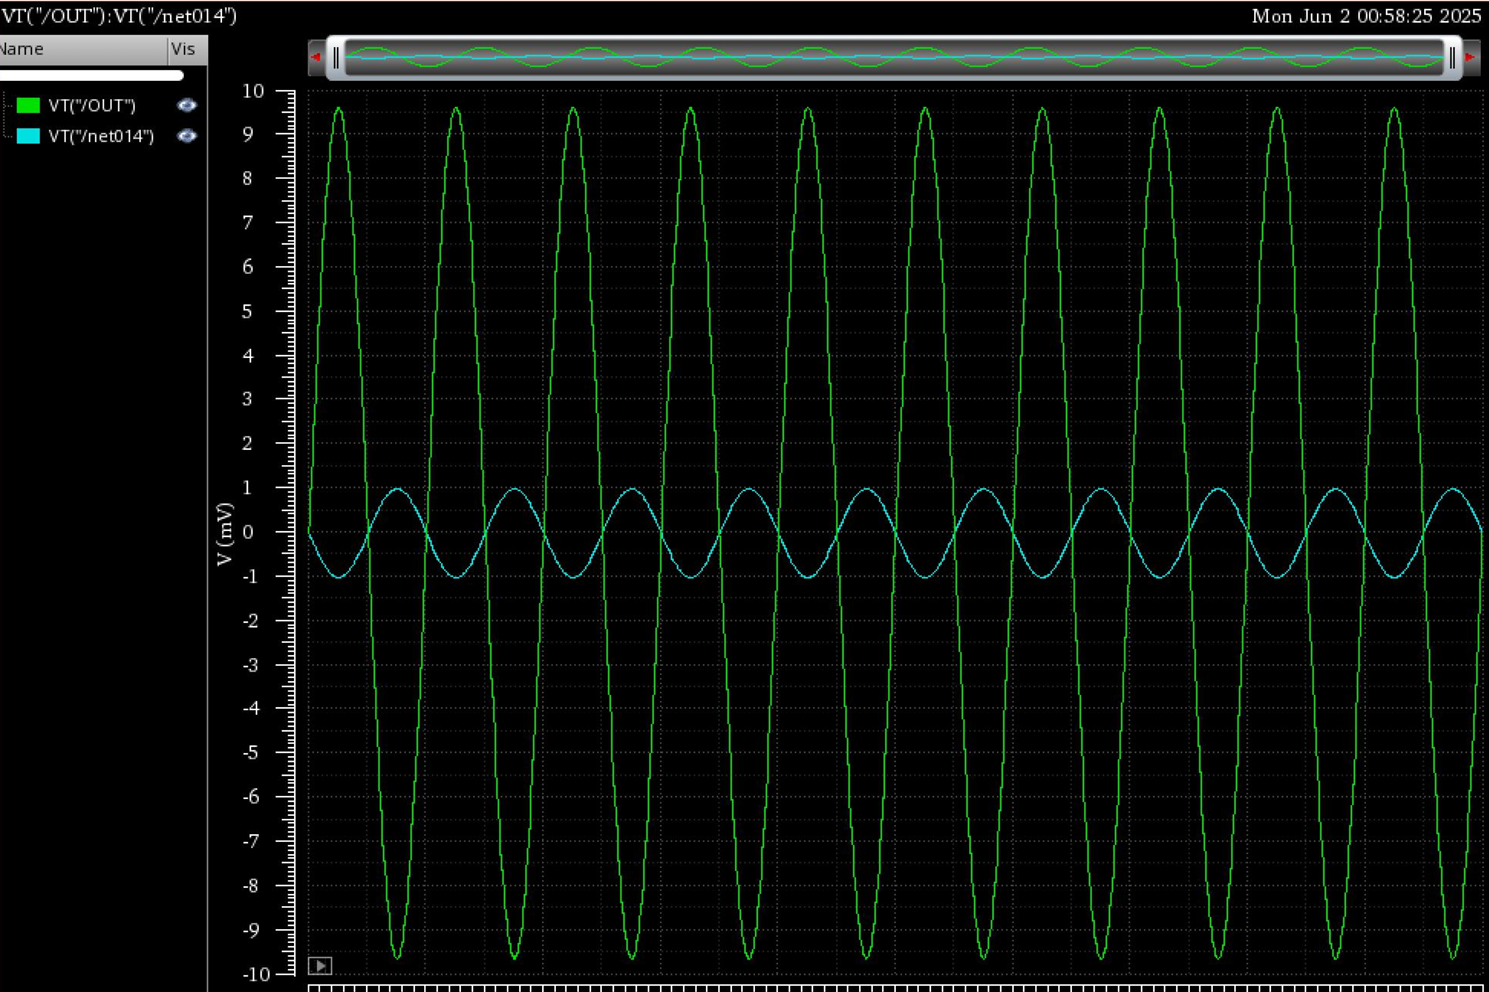
\includegraphics[width=0.8\textwidth]{chapters/figure/A12/A12ten.png}
\caption{电压放大倍数仿真结果}
\label{电压放大倍数仿真结果}
\end{figure}

\tt{仿真得到电压放大倍数为-9.57（图中9.41并非顶峰），大致满足设计要求}

\begin{figure}[H]
\centering
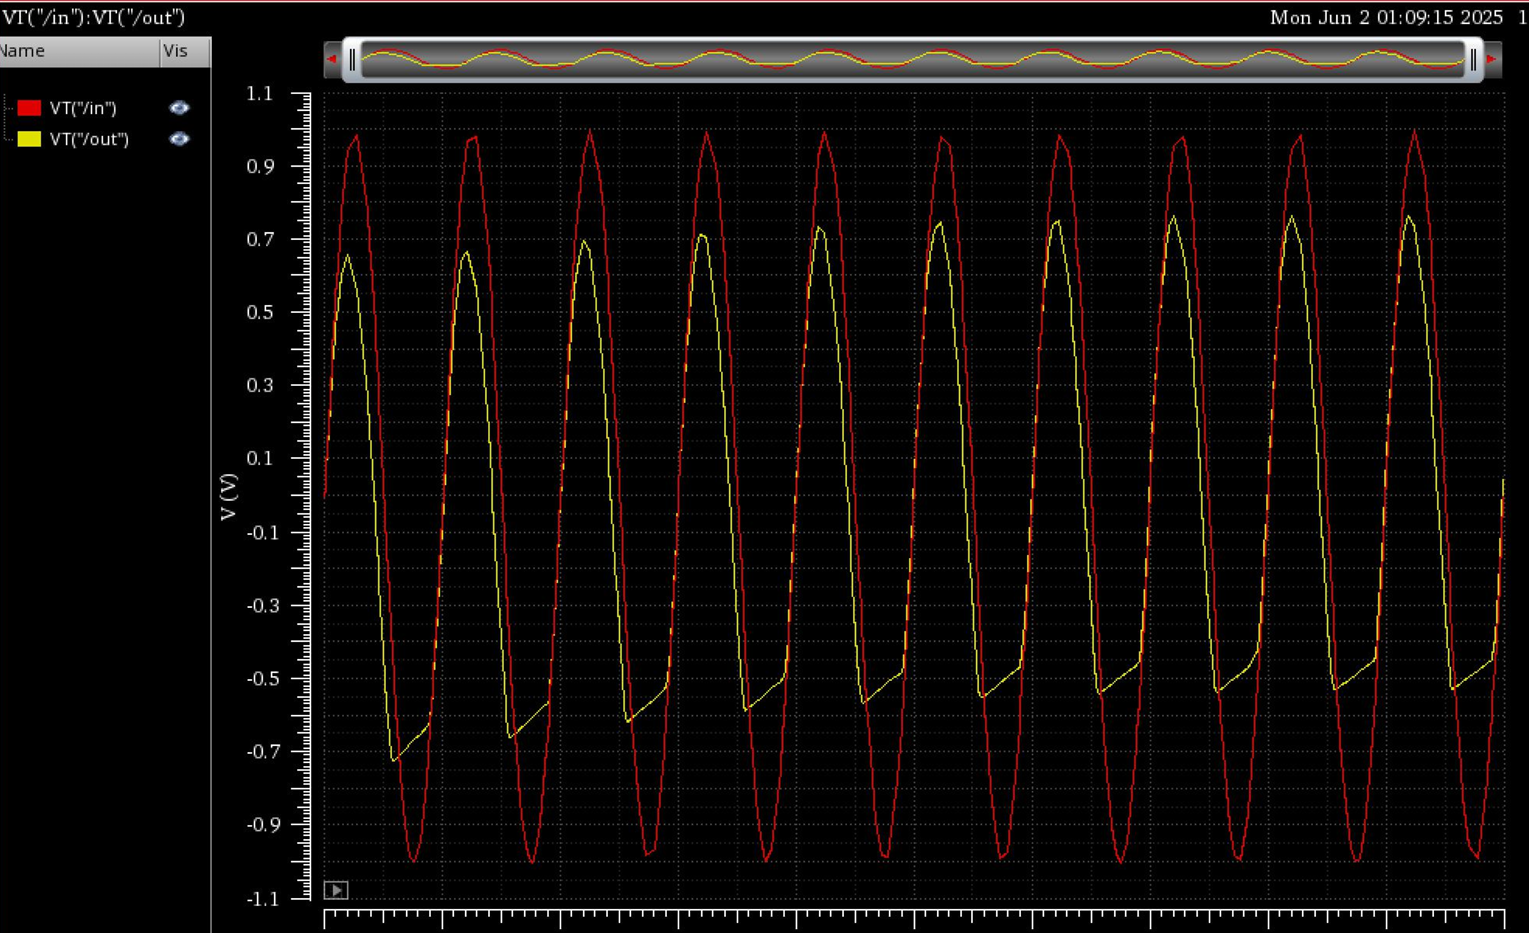
\includegraphics[width=0.8\textwidth]{chapters/figure/A12/A121V.png}
\caption{输入电压不为小信号的失真}
\label{输入电压不为小信号的失真}
\end{figure}
\tt{当输入电压不为小信号时，输出波形失真，无法满足要求}

\begin{figure}[H]
\centering
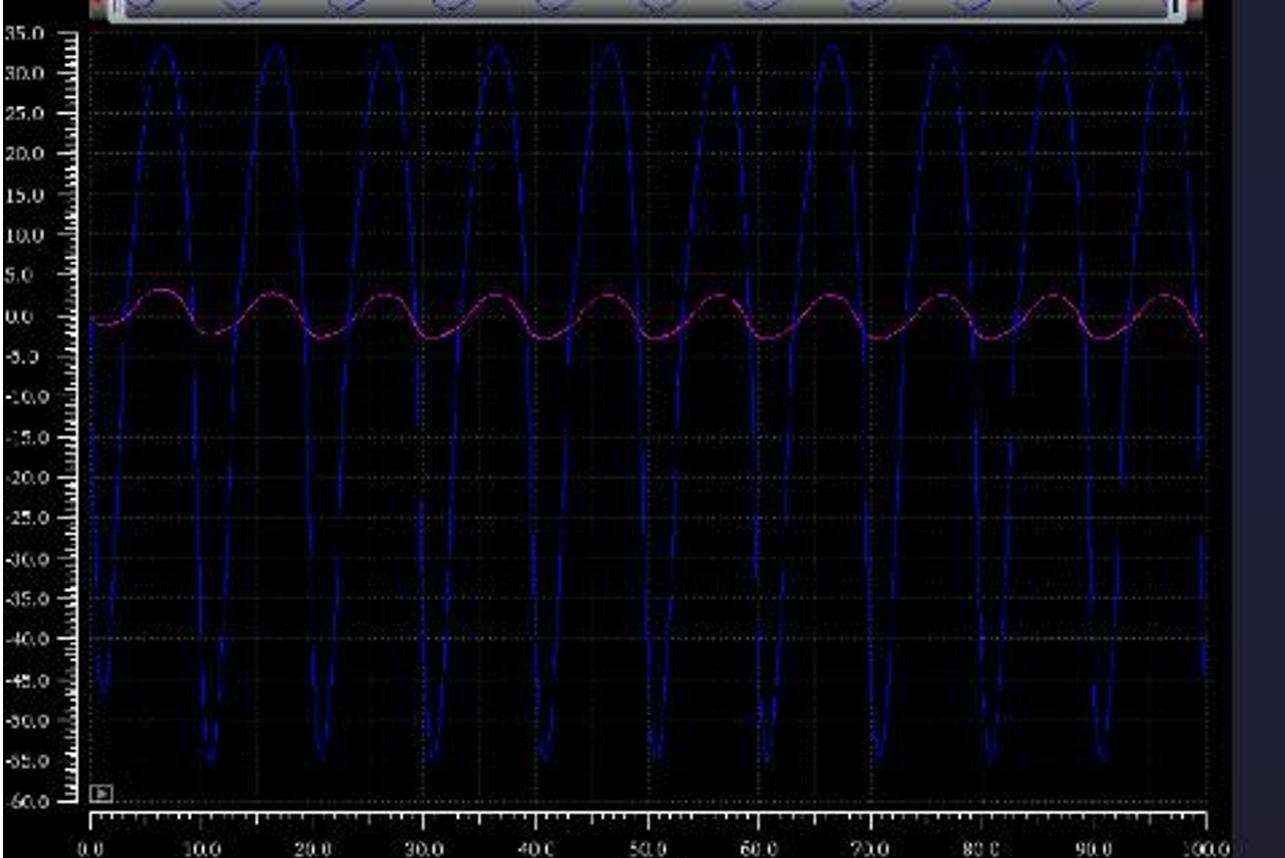
\includegraphics[width=0.8\textwidth]{chapters/figure/A12/1kHz.png}
\caption{1kHz输入电压的失真}
\label{1kHz输入电压的失真}
\end{figure}
\tt{当输入频率为1kHz时，输出波形增益改变，无法满足要求}

\subsection{100倍增益：}
\tt{可以通过bjt常用的达林顿接法实现100倍增益}

\begin{figure}[H]
\centering
\resizebox{1\textwidth}{!}{%
\begin{circuitikz}
\tikzstyle{every node}=[font=\large]
\draw (2.5,11.25) to[american voltage source] (2.5,9);
\draw (2.5,11.25) to[european resistor,l={ \normalsize $R_{S}=100\Omega$}] (4.75,11.25);
\draw (4.75,11.25) to[C,l={ \normalsize $C_{B}=10uF$}] (6,11.25);
\draw (6.5,12.5) to[european resistor,l={ \normalsize $R_{B1}=20k\Omega$}] (6.5,15.25);
\draw (6.5,10) to[european resistor,l={ \normalsize $R_{B2}=20k\Omega$}] (6.5,7.5);
\draw (9,10) to[Tnpn, transistors/scale=1.19] (9,12.5);
\draw (9,12.5) to[european resistor,l={ \normalsize $R_{C}=500\Omega$}] (9,15.25);
\draw (2.5,9.25) to[short] (2.5,7.5);
\draw (2.5,7.5) to[short] (12.5,7.5);
\draw (5.75,11.25) to[short] (8,11.25);
\draw (6.5,12.5) to[short] (6.5,11.25);
\draw (6.5,15.25) to[short] (9,15.25);
\draw (6.5,11.25) to[short] (6.5,9.75);
\draw (9,15.25) to[short, -o] (9,16) ;
\draw (9.75,16) to[short, -o] (9.75,16) node {5V};
\draw (13.75,7.5) to[short] (11.75,7.5);
\draw (10.5,9) to[Tnpn, transistors/scale=1.19] (10.5,11);
\draw (9,10) to[short] (9.5,10);
\draw (10.5,9.25) to[european resistor,l={ \normalsize $30\Omega$}] (10.5,7.5);
\draw (10.5,15.25) to[L,l={ \normalsize $2.71mH$} ] (10.5,12.75);
\draw (9,15.25) to[short] (10.5,15.25);
\draw (10.5,13.25) to[short] (10.5,10.75);
\draw (10.5,11.75) to[C,l={ \normalsize $10uF$}] (12.75,11.75);
\draw (13.75,11.25) to[european resistor,l={ \normalsize $1k\Omega$}] (13.75,7.5);
\draw (12.75,11.75) to[short] (13.75,11.75);
\draw (13.75,11.75) to[short] (13.75,10.75);
\end{circuitikz}
}%

\label{fig:my_label}
\end{figure}

\begin{figure}[H]
\centering
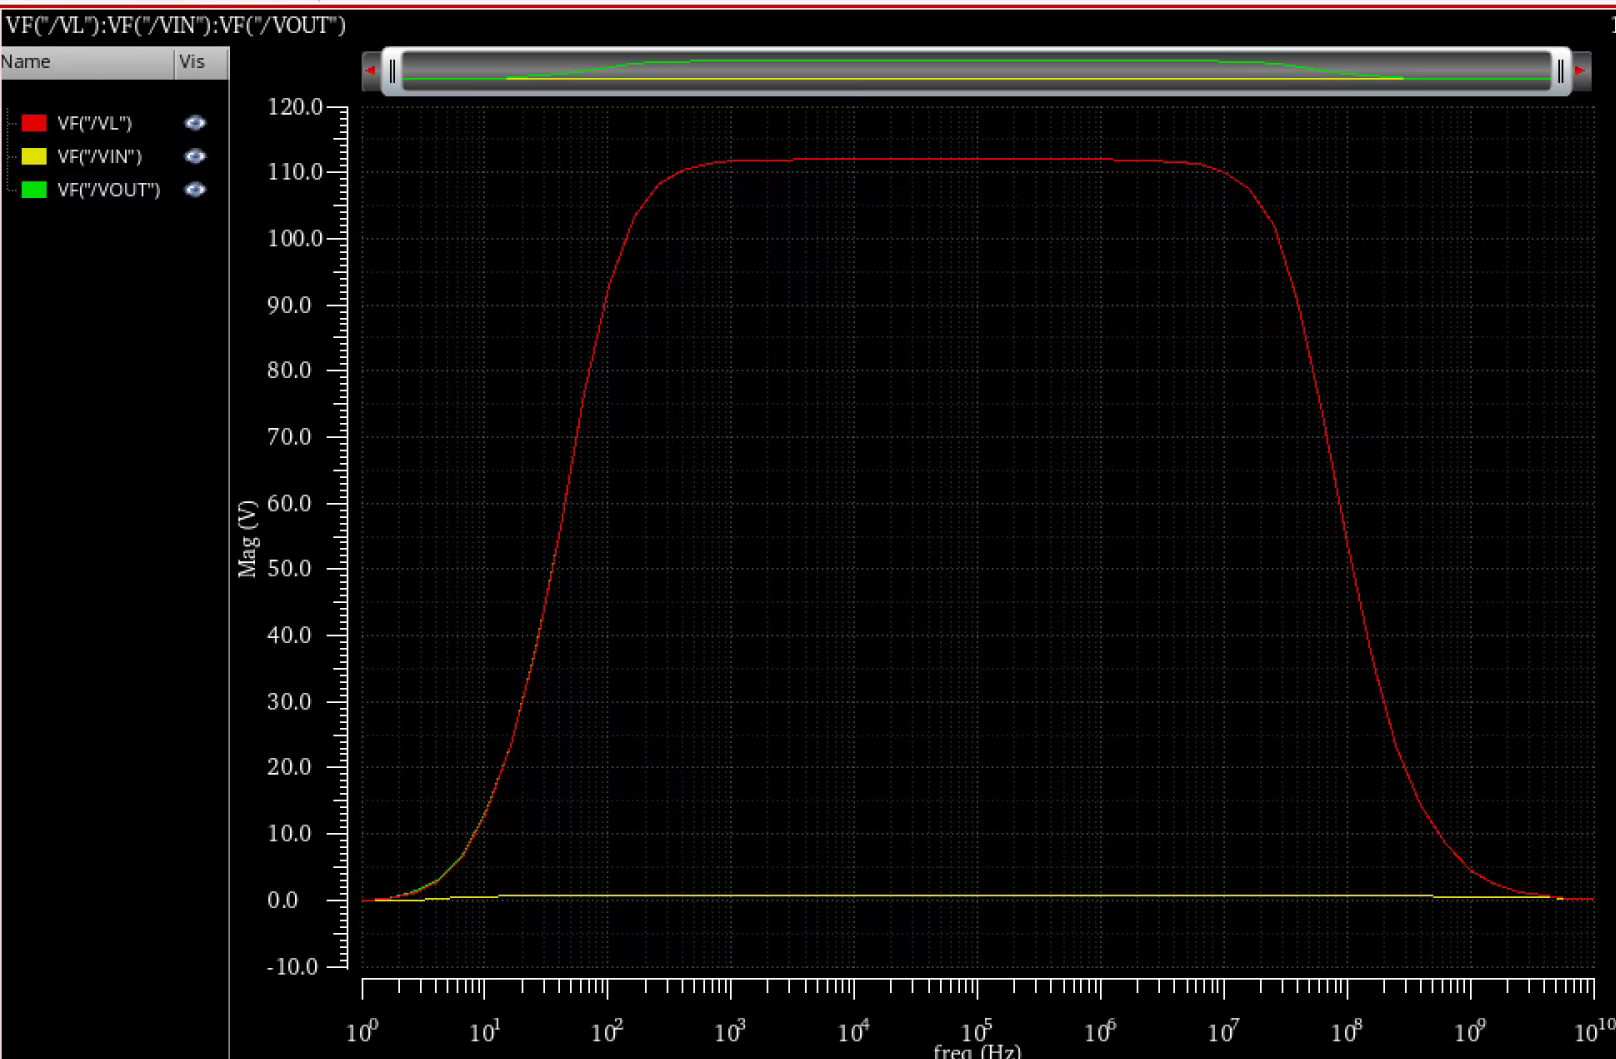
\includegraphics[width=0.8\textwidth]{chapters/figure/A12/100.png}
\caption{达林顿接法实现100倍增益}
\label{达林顿接法实现100倍增益}
\end{figure}
\tt{放大倍数大约110倍，且比较稳定，符合要求}